\taskpic{ Два диска одинакового радиуса вращаются в одном направлении
  с одинаковой угловой скоростью $\omega_0$. Их приводят в контакт, и
  затем система через некоторое время приходит в новое установившееся
  состояние движения. Моменты инерции дисков относительно их осей
  вращения равны $I_1$ и $I_2$, трения в осях нет. Найти изменение
  момента импульса системы и её кинетической энергии.}
{
  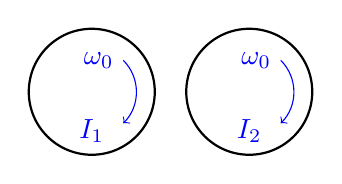
\begin{tikzpicture}
    \draw[thick] (1,1) circle (0.8cm);
    \draw[thick] (3,1) circle (0.8cm);
    \draw[blue] (1,0.5) node{$I_1$};
    \draw[blue] (3,0.5) node{$I_2$};
    \draw[blue,->] (1.4,1.4) node[left] {$\omega_0$}
    arc(45:-45:sqrt{0.32});
    \draw[blue,->] (3.4,1.4) node[left] {$\omega_0$}
    arc(45:-45:sqrt{0.32});
  \end{tikzpicture}
}
% Паршаков, 2.2.28